\section{Ejercicio 7}
\subsection{Enunciado}

\subsection{Soluci\'on}

%SI QUIEREN AGREGAR IMAGENES COPIEN EL SIGUIENTE CODIGO
%\begin {center}
%\includegraphics[width=12cm]{./graphEj1.jpg}
% grafico.eps: 0x0 pixel, 300dpi, 0.00x0.00 cm, bb=50 50 410 302
%\end {center}

Lote simulado con Round Robin:

\verbatiminput{../simusched/lotes/loteEj7.tsk}

\par Diagrama con 2 ciclos de quantum:

\begin {center}
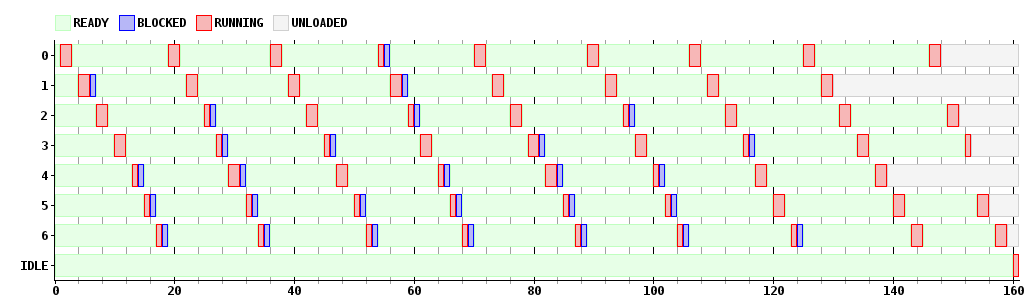
\includegraphics[width=12cm]{../simusched/outputs/ej7/rr-ej7-1-2.png}
\end {center}

\par Diagrama con 5 ciclos de quantum:
\begin {center}
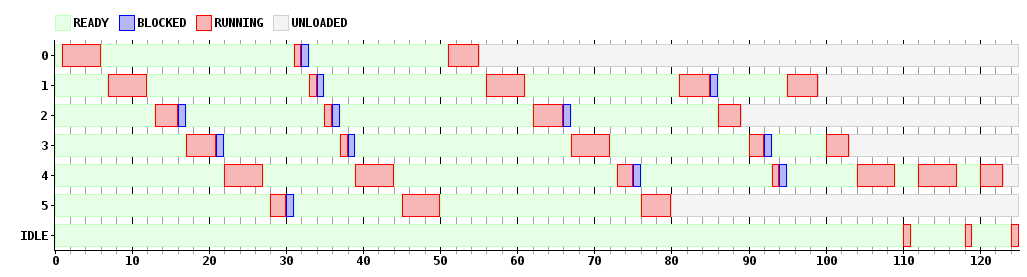
\includegraphics[width=12cm]{../simusched/outputs/ej7/rr-ej7-1-5.png}
\end {center}

\par Diagrama con 7 ciclos de quantum:
\begin {center}
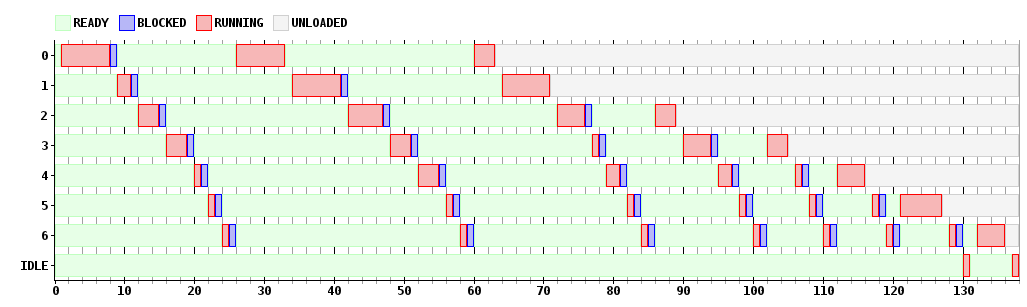
\includegraphics[width=12cm]{../simusched/outputs/ej7/rr-ej7-1-7.png}
\end {center}

\par Diagrama con 9 ciclos de quantum:
\begin {center}
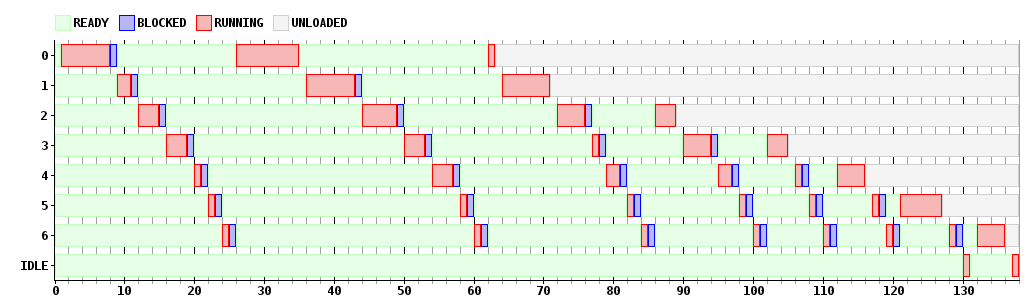
\includegraphics[width=12cm]{../simusched/outputs/ej7/rr-ej7-1-9.png}
\end {center}

\par Diagrama con 12 ciclos de quantum:
\begin {center}
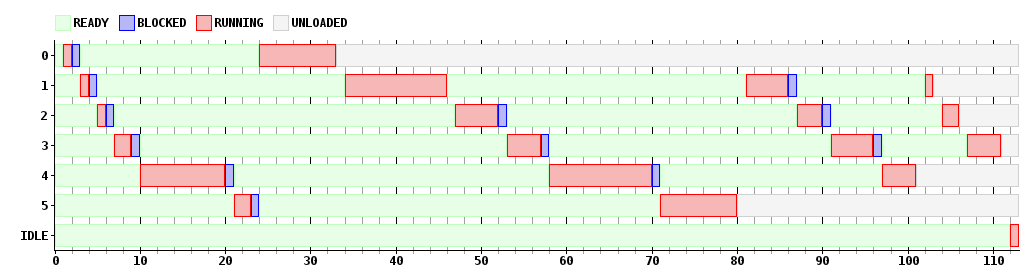
\includegraphics[width=12cm]{../simusched/outputs/ej7/rr-ej7-1-12.png}
\end {center}

\par Diagrama con 17 ciclos de quantum:
\begin {center}
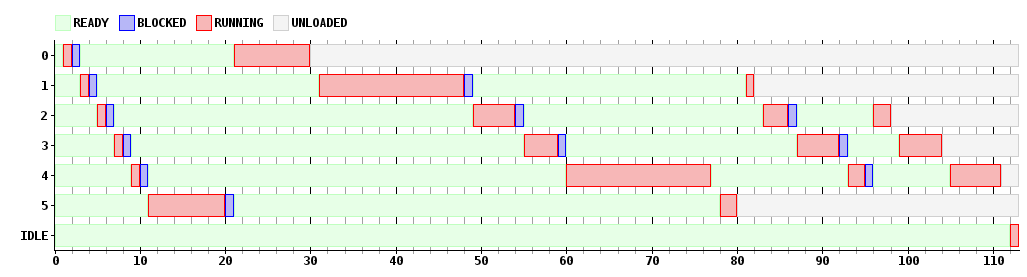
\includegraphics[width=12cm]{../simusched/outputs/ej7/rr-ej7-1-17.png}
\end {center}

\par Diagrama con 21 ciclos de quantum:
\begin {center}
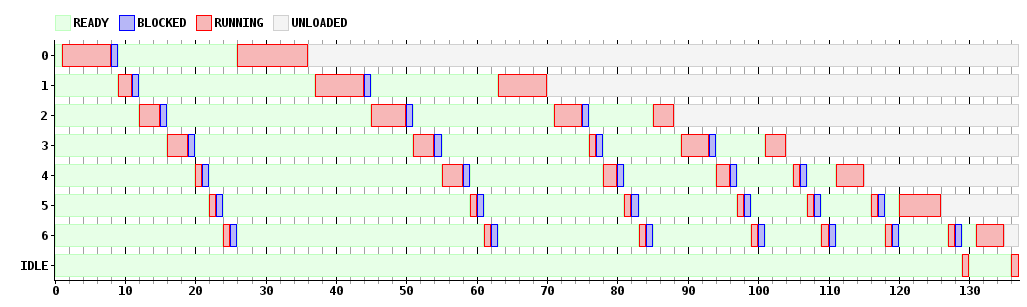
\includegraphics[width=12cm]{../simusched/outputs/ej7/rr-ej7-1-21.png}
\end {center}

Se puede observar que a medida que los ciclos del quantum aumentan, las tareas van finalizan más rapido, debido a que se le da mas tiempo de ejecución, hay una menor cambio de contexto entre los procesos y ocurren menos bloqueos por intervalo de ejecución del proceso.
\\
Para este lote de tareas en general, suele ser mas eficiente asignarle una cantidad grande de ciclos por quantum,  ya que se realizarán menos bloqueos y cada proceso podrá finalizar en la menor cantidad de $"$cortes$"$ de ejecución, pero no excesiva, porque, como se aprecia en las imágenes, entre 12 y 21  ciclos por quantum todos tardan lo mismo en finalizar y no mejora la eficiencia.
\\
Con un quantum de 21 ciclos, se puede notar que lo que mas influye en cada proceso son los bloqueos que se producen y no tanto el corte porque no le quedan mas ciclos, produciendo cambios de contexto obligatorios y empeorando bastante la optimización del Round Robin frente a otros algoritmos de scheduling.


